\documentclass[a4paper,12pt]{article}
\usepackage[utf8]{inputenc}
\usepackage{geometry}
\usepackage{listings}
\usepackage{xcolor}
\usepackage{hyperref}
\geometry{margin=1in}
\usepackage{graphicx}

\title{Couche Contrôleur}
\date{\today}

\lstset{
  basicstyle=\ttfamily\small,
  keywordstyle=\color{blue}\bfseries,
  stringstyle=\color{red},
  commentstyle=\color{gray},
  breaklines=true,
  frame=single,
}

\begin{document}

\maketitle

\section{Comprendre la Couche Contrôleur et les Tests d'Inté-gration dans Spring Boot}

\subsection{Introduction à la Couche Contrôleur}
La \textit{couche contrôleur} est une partie essentielle d'une application Spring Boot. Elle gère les requêtes HTTP des clients et les associe aux services ou à la logique métier appropriés. Grâce aux contrôleurs, nous définissons les \textit{endpoints} de notre API REST, permettant aux clients d'effectuer des opérations comme la création, la lecture, la mise à jour ou la suppression de ressources.

\subsubsection{Rôle de la Couche Contrôleur}
\begin{itemize}
    \item Agit comme une \textit{passerelle} vers l'application.
    \item Transforme les requêtes client en appels de service appropriés.
    \item Gère à la fois les données entrantes (corps des requêtes) et les réponses sortantes (renvoyées au client).
    \item Garantit que l'application respecte les principes de l'architecture RESTful.
\end{itemize}

\subsubsection{Annotations Clés dans les Contrôleurs}
\begin{itemize}
    \item \texttt{@RestController} : Marque une classe comme un contrôleur où chaque méthode renvoie un corps de réponse.
    \item \texttt{@RequestMapping} : Associe des requêtes HTTP à des méthodes ou des classes spécifiques.
    \item \texttt{@PostMapping}, \texttt{@GetMapping}, \texttt{@PutMapping}, \texttt{@DeleteMapping} : Associent des méthodes HTTP (POST, GET, PUT, DELETE) à des opérations spécifiques.
    \item \texttt{@RequestBody} : Lie le corps d'une requête client à un paramètre de méthode.
    \item \texttt{@PathVariable} : Extrait une valeur de l'URI pour l'utiliser dans la méthode.
    \item \texttt{@Autowired} : Injecte des dépendances comme des services dans le contrôleur.
\end{itemize}
\noindent\begin{figure}[h!]
    \centering
    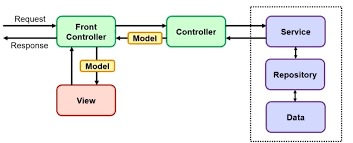
\includegraphics[width=\textwidth]{images/controller_layer01.jpg}
    \caption{Diagramme de la Couche Contrôleur interagissant avec d'autres composants tels que les Services, les Référentiels et les Clients.}
    \label{fig:controller_layer_diagram}
\end{figure}

\section{Les Contrôleurs que Nous Avons Construits}
\subsection{Contrôleur Auteur}
\textbf{Objectif} : Gérer les auteurs avec des détails comme \texttt{nom} et \texttt{âge}.
\begin{itemize}
    \item \textbf{Endpoints} :
    \begin{itemize}
        \item \textbf{Créer} : \texttt{POST /api/authors/save} - Ajoute un nouvel auteur au système.
        \item \textbf{Lire} :
        \begin{itemize}
            \item \texttt{GET /api/authors/all} : Récupère tous les auteurs.
            \item \texttt{GET /api/authors/one/\{id\}} : Récupère un auteur spécifique par ID.
        \end{itemize}
        \item \textbf{Mettre à jour} : \texttt{PUT /api/authors/update/\{id\}} - Modifie les détails d'un auteur.
        \item \textbf{Supprimer} : \texttt{DELETE /api/authors/delete/\{id\}} - Supprime un auteur par ID.
    \end{itemize}
\end{itemize}

\textbf{Exemple de Code : Contrôleur Auteur}
L'exemple suivant montre l'implémentation d'une couche contrôleur (Contrôleur Auteur).
Il contient les annotations et toutes les fonctionnalités requises pour cette couche.

Le code complet est disponible dans le dépôt GitHub du projet : 
\hspace{5}\
\vspace{0.1cm}\

\url{https://github.com/D0esN0tM1tter/spring_boot_project-/blob/master/supporting_project/supporting_project/src/main/java/com/example/demo/controllers/AuthorController.java}.

\vspace{0.5cm}\

\textbf{Explication} :
\begin{itemize}
    \item La classe est annotée avec \texttt{@RestController}, indiquant qu'elle gère les requêtes HTTP et fournit des réponses au format JSON.
    \item L'annotation \texttt{@PostMapping("/save")} spécifie l'endpoint pour enregistrer un auteur.
    \item \texttt{AuthorService} est injecté en utilisant \texttt{@Autowired} pour gérer la logique métier.
    \item La méthode \texttt{create()} prend un objet \texttt{AuthorDto}, appelle la couche service pour l'enregistrer, et renvoie une réponse avec le statut \texttt{201 CREATED}.
\end{itemize}

\subsection{Contrôleur Livre}
\textbf{Objectif} : Gérer les livres avec des attributs comme \texttt{titre}, \texttt{auteur}, \texttt{catégorie} et \texttt{date de publication}.
\begin{itemize}
    \item \textbf{Endpoints} :
    \begin{itemize}
        \item \textbf{Créer} : \texttt{POST /api/books/save} - Ajoute un nouveau livre.
        \item \textbf{Lire} :
        \begin{itemize}
            \item \texttt{GET /api/books/all} : Récupère tous les livres.
            \item \texttt{GET /api/books/one/\{id\}} : Récupère un livre spécifique par ID.
        \end{itemize}
        \item \textbf{Mettre à jour} : \texttt{PUT /api/books/update/\{id\}} - Met à jour les détails d'un livre.
        \item \textbf{Supprimer} : \texttt{DELETE /api/books/delete/\{id\}} - Supprime un livre.
    \end{itemize}
\end{itemize}

\textbf{Exemple de Code : Tests d'intégration du Contrôleur Livre}

L'exemple suivant démontre l'implémentation d'un test d'intégration pour la couche contrôleur.  
Il inclut les annotations nécessaires ainsi que toute la logique JUnit et MockMvc requise pour cette couche.

Le code complet est disponible sur le dépôt GitHub du projet :  
\hspace{5}\\

\url{https://github.com/D0esN0tM1tter/spring_boot_project-/blob/master/supporting_project/supporting_project/src/test/java/com/example/demo/services/BookServicesIntegrationTests.java}.

\section{Contrôleur Catégorie}
\textbf{Objectif} : Gérer les catégories qui classifient les livres.
\begin{itemize}
    \item \textbf{Points de terminaison} :
    \begin{itemize}
        \item \textbf{Créer} : \texttt{POST /api/category/save} - Ajoute une nouvelle catégorie.
        \item \textbf{Lire} :
        \begin{itemize}
            \item \texttt{GET /api/category/all} : Liste toutes les catégories.
            \item \texttt{GET /api/category/one/\{id\}} : Récupère une catégorie spécifique par ID.
        \end{itemize}
        \item \textbf{Mettre à jour} : \texttt{PUT /api/category/update/\{id\}} - Met à jour les détails d'une catégorie.
        \item \textbf{Supprimer} : \texttt{DELETE /api/category/delete/\{id\}} - Supprime une catégorie.
    \end{itemize}
\end{itemize}

\section{Tests d'Intégration : MockMvc et Transformation JSON-DTO-Entity}

\subsection{Pourquoi les tests sont importants}
Les tests permettent de vérifier que :
\begin{itemize}
    \item Chaque contrôleur gère les requêtes comme prévu.
    \item Les données circulent correctement entre les contrôleurs et les services.
    \item Le système répond correctement aux erreurs ou aux entrées invalides.
\end{itemize}

\subsection{Options de tests et pourquoi nous avons choisi MockMvc}
Lors du développement d'une application web, plusieurs options de tests sont disponibles. Par exemple, des tests peuvent être effectués côté serveur avec des technologies telles que JPA, Thymeleaf, ou en utilisant des frameworks frontend comme Angular pour tester l'interaction entre le client et le serveur.

\subsection{Approches possibles pour les tests}
\begin{itemize}
    \item \textbf{Tests côté serveur (JPA, Thymeleaf)} : 
    \begin{itemize}
        \item Les tests côté serveur impliquent de tester la logique métier dans le backend. Par exemple, JPA (Java Persistence API) peut être utilisé pour tester les interactions avec la base de données, en s'assurant que les entités sont correctement persistées et récupérées. 
        \item Thymeleaf, intégré avec Tomcat, peut être utilisé pour tester la génération côté serveur de vues en utilisant des modèles HTML dynamiques. Ces tests vérifient que les données sont correctement injectées dans les pages HTML avant leur rendu.
    \end{itemize}
    
    \item \textbf{Tests avec des frameworks Front-End (Angular)} : 
    \begin{itemize}
        \item Un autre type de test consiste à tester les interactions entre le frontend et le backend. Des frameworks comme Angular permettent de simuler des requêtes HTTP et de vérifier que le serveur répond correctement aux actions des utilisateurs. Ces tests vérifient non seulement l'intégration du frontend avec le backend mais aussi l'interface utilisateur et les interactions avec l'API.
    \end{itemize}
\end{itemize}

\subsection{Pourquoi nous avons choisi MockMvc}
Bien que d'autres méthodes de test puissent être utilisées pour tester l'application de bout en bout, nous avons choisi d'utiliser \texttt{MockMvc} pour nos tests d'intégration. Cette approche présente plusieurs avantages, notamment :
\begin{itemize}
    \item \textbf{Test simplifié du Backend} : \texttt{MockMvc} nous permet de simuler des requêtes HTTP directement sur le contrôleur sans nécessiter un serveur réel comme Tomcat. Cela permet de tester l'intégration des couches contrôleur et service sans avoir besoin d'une configuration complète de serveur ou d'un client frontend comme Angular.
    \item \textbf{Vérification de la logique métier} : Avec \texttt{MockMvc}, nous pouvons vérifier que la logique métier, le routage des requêtes et la transformation des données (via les DTO, entités, etc.) fonctionnent comme prévu, tout en évitant les complexités supplémentaires liées à la configuration d'un serveur web complet ou d'un framework frontend.
    \item \textbf{Isolation et concentration sur l'API} : Cette méthode permet de tester uniquement l'API, isolant le backend sans avoir besoin d'un client frontend. Cela rend les tests plus rapides et plus ciblés, en nous concentrant sur les composants essentiels côté serveur.
\end{itemize}

En résumé, bien que des alternatives telles que JPA, Thymeleaf ou des tests avec Angular existent pour tester les interactions entre différents composants, l'utilisation de \texttt{MockMvc} nous permet de tester efficacement le backend en isolation et de nous concentrer sur la logique backend, tout en simplifiant le processus de test.

\subsection{Rôle de MockMvc}

\subsubsection{Qu'est-ce que MockMvc ?}
MockMvc est un outil de Spring qui permet de tester des contrôleurs sans démarrer un serveur. Il simule des requêtes HTTP et fournit des réponses comme dans une véritable interaction client-serveur.
\subsubsection{Pourquoi MockMvc ?}
\begin{itemize}
    \item Évite la nécessité d'un serveur en fonctionnement.
    \item Simule le processus de requête et réponse HTTP.
    \item Idéal pour les tests d'intégration puisqu'il garantit que le contrôleur interagit correctement avec la couche de service et les autres composants.
\end{itemize}

\subsubsection{Étapes pour tester avec MockMvc :}
\begin{itemize}
    \item Configurer MockMvc avec \texttt{@AutoConfigureMockMvc} dans votre classe de test.
    \item Utiliser MockMvc pour simuler des requêtes HTTP (par exemple, POST, GET).
    \item Vérifier les codes de statut, les en-têtes et le corps des réponses attendues.
\end{itemize}

\subsection{Exemple MockMvc : Tests du BookController}
\subsubsection{Test pour la création d'un livre}
\textit{Simule une requête POST pour créer un nouveau livre. Convertit un objet BookDto en JSON, envoie la charge utile JSON via MockMvc, et vérifie le code de statut (201 Créé) et le contenu de la réponse (par exemple, titre, auteur).}

\newpage
\begin{lstlisting}[language=Java]
@Test
public void testCreateBook() throws Exception {
    AuthorDto author = new AuthorDto("Sami", 21);
    CategoryDto category = new CategoryDto("Info");
    BookDto book = new BookDto("Java", author, category, parseDate("2024-11-20"));

    String bookJson = objectMapper.writeValueAsString(book);

    mockMvc.perform(MockMvcRequestBuilders.post("/api/books/save")
            .contentType(MediaType.APPLICATION_JSON)
            .content(bookJson))
            .andExpect(MockMvcResultMatchers.status().isCreated())
            .andExpect(MockMvcResultMatchers.jsonPath("$.title").value("Java"))
            .andExpect(MockMvcResultMatchers.jsonPath("$.author.name").value("Sami"));
}
\end{lstlisting}
\subsubsection{Test de la recherche d'un livre par ID}
\begin{itemize}
    \item Simule une requête GET pour récupérer un livre par ID.
    \item Vérifie le statut de la réponse (200 OK) et le contenu (par exemple, le titre du livre, l'auteur).
\end{itemize}

\subsubsection{Test de la recherche de tous les livres}
\begin{itemize}
    \item Simule une requête GET pour récupérer tous les livres.
    \item Vérifie la liste des livres dans la réponse.
\end{itemize}

\subsubsection{Intégration de MockMvc dans la classe de test}
\begin{itemize}
    \item \texttt{@SpringBootTest} : Charge l'ensemble du contexte de l'application pour les tests.
    \item \texttt{@AutoConfigureMockMvc} : Active MockMvc pour les tests d'intégration.
    \item \texttt{MockMvc.perform} : Exécute les requêtes HTTP.
    \item \texttt{ObjectMapper} : Sérialise les objets Java en JSON et vice versa.
\end{itemize}

\subsection{3.3.2 Pourquoi des tests d'intégration ?}
Les tests d'intégration valident l'interaction entre :
\begin{itemize}
    \item \textbf{Les couches Contrôleur et Service}.
    \item \textbf{Les DTO, Entités et JSON}.
\end{itemize}

\section{Utilité de la transformation JSON-DTO-Entité dans un projet en couches}

\subsection{Transformation JSON-DTO-Entité}

Dans notre projet en couches, la \textbf{transformation JSON-DTO-Entité} est un patron de conception essentiel qui garantit un flux de données propre entre les différentes couches de l'application.

\begin{itemize}
    \item \textbf{JSON} :
    \begin{itemize}
        \item Représente les données échangées entre le client et le serveur.
        \item Utilisé comme format standard pour les corps des requêtes et des réponses HTTP en raison de sa simplicité et de sa lisibilité.
    \end{itemize}
    \item \textbf{DTO (Data Transfer Object)} :
    \begin{itemize}
        \item Sert d'intermédiaire entre le client et les couches internes de l'application.
        \item Permet la validation et la structuration des données entrantes et sortantes sans exposer la structure de la base de données.
        \item Prévient le couplage étroit entre les API externes et les modèles internes du domaine.
    \end{itemize}
    \item \textbf{Entité} :
    \begin{itemize}
        \item Représente la structure réelle de la base de données utilisée pour la persistance.
        \item La couche Service convertit les DTO en Entités pour les opérations sur la base de données et inversement.
    \end{itemize}
\end{itemize}

\noindent\begin{figure}[h!]
    \centering
    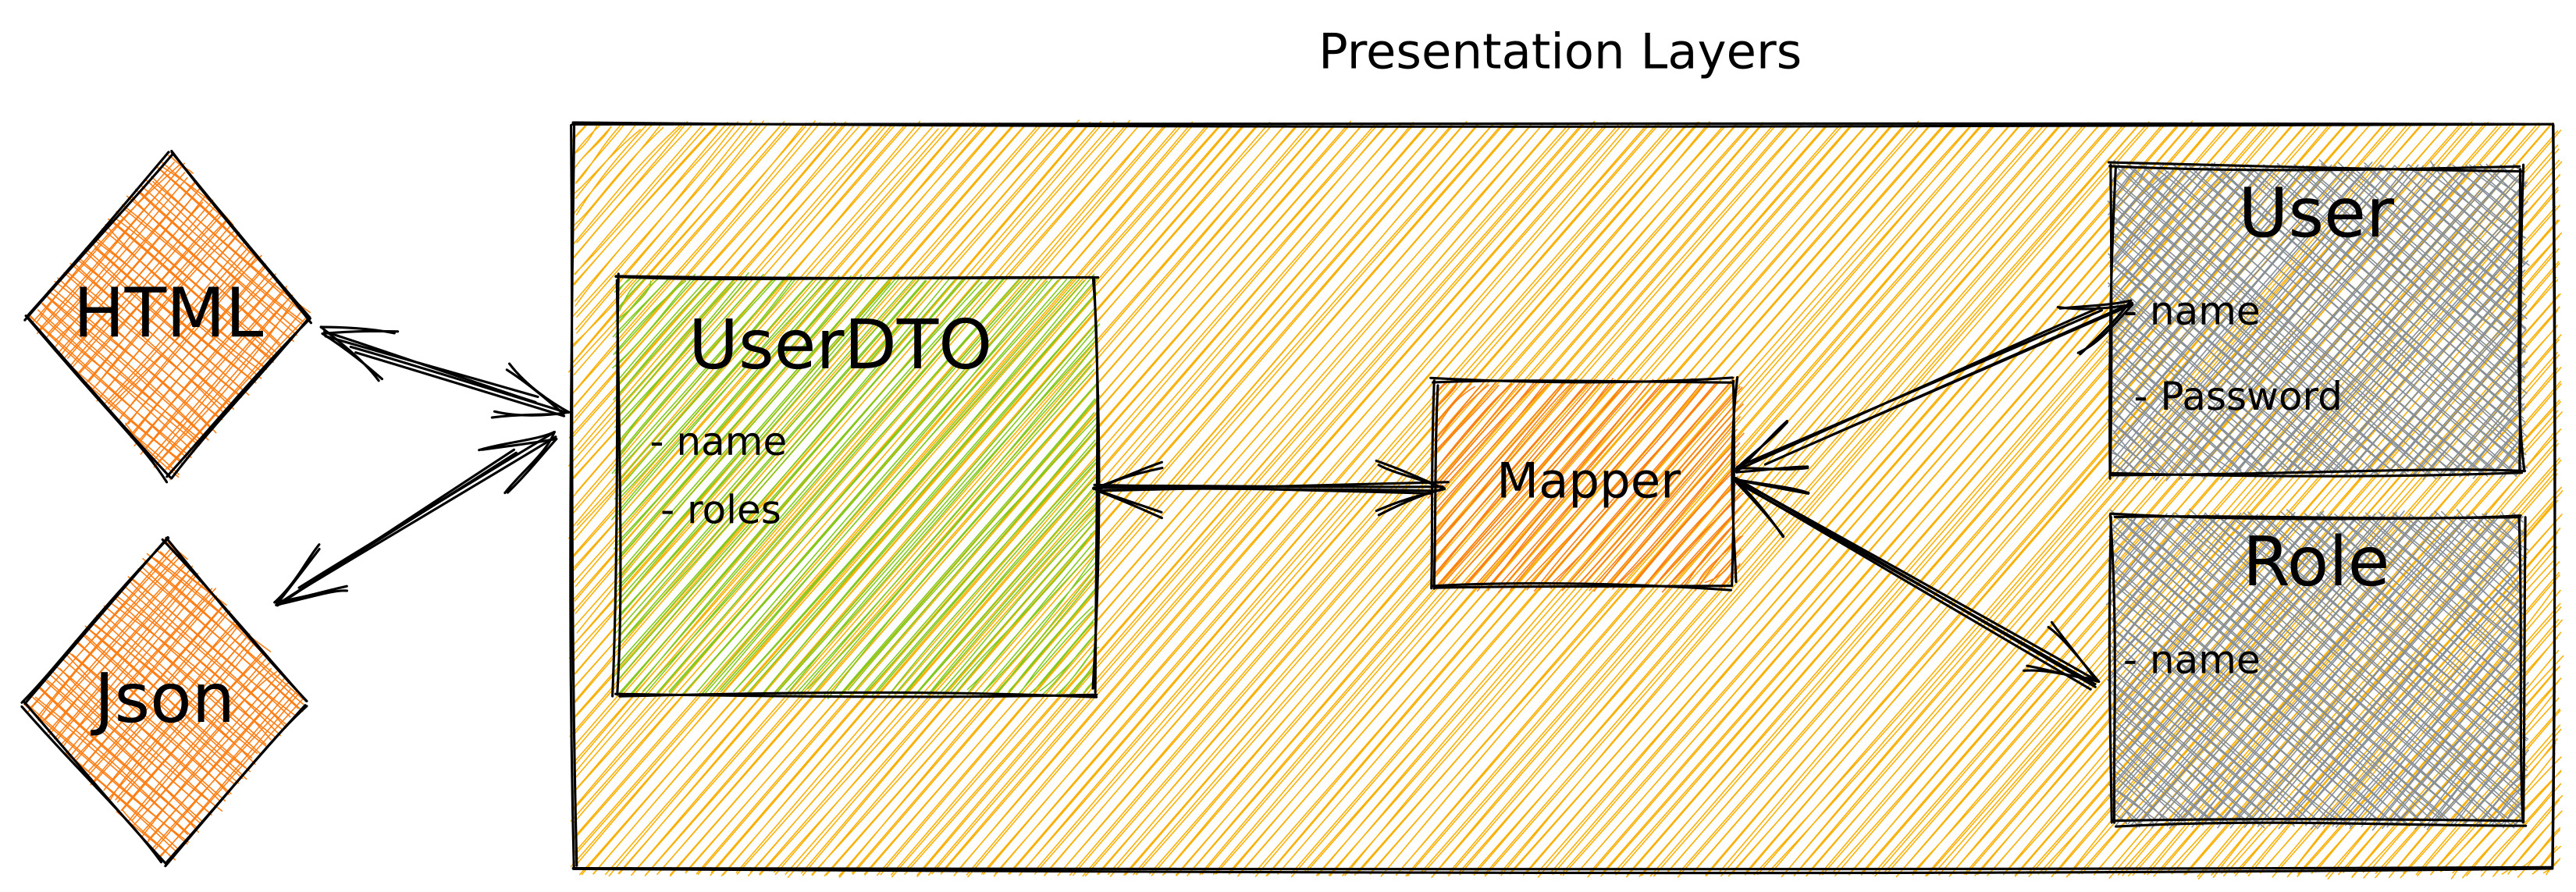
\includegraphics[width=\textwidth]{images/layers-4.jpg}
    \caption{Ajoutez un diagramme montrant la transformation de JSON $\rightarrow$ DTO $\rightarrow$ Entité.}
    \label{fig:Transformation_JSON_DTO_Entity_diagram}
\end{figure}

\section{Comprendre l'architecture REST}

Le \textit{Representational State Transfer} (REST) est un style architectural utilisé pour concevoir des applications en réseau. REST repose sur les principes de l'absence d'état, des interactions orientées ressources et de l'utilisation des méthodes HTTP standard.

Les applications RESTful exposent leurs ressources via des Identifiants Uniformes de Ressources (URI) et permettent l'interaction avec ces ressources à l'aide des verbes HTTP suivants :
\begin{itemize}
    \item \textbf{GET} : Récupérer une ressource ou une liste de ressources.
    \item \textbf{POST} : Créer une nouvelle ressource.
    \item \textbf{PUT} : Mettre à jour une ressource existante.
    \item \textbf{DELETE} : Supprimer une ressource.
\end{itemize}

Un système RESTful communique en utilisant un protocole sans état, généralement HTTP, ce qui assure évolutivité et simplicité. Les données sont souvent échangées dans des formats comme JSON ou XML, ce qui les rend légères et compatibles avec différents types de clients.

REST joue un rôle essentiel dans le développement des applications web modernes en permettant des interactions flexibles et efficaces entre les clients et les serveurs.

\subsection{REST dans le contexte du projet}

Dans ce projet, REST a été choisi pour concevoir des API facilitant la communication entre le client et le serveur. Ces API gèrent des ressources telles que les données des utilisateurs, les tâches ou les transactions, en suivant les principes REST. En adoptant REST, l'application bénéficie d'une meilleure modularité, d'une intégration facilitée avec les systèmes tiers et d'interactions client-serveur simplifiées.

\subsection{Tester les API RESTful avec MockMvc}

Les API RESTful mises en œuvre dans ce projet ont été testées à l'aide de \texttt{MockMvc}, un framework fourni par Spring pour tester les applications web. En utilisant \texttt{MockMvc}, nous avons assuré que les API respectaient les principes REST et renvoyaient les résultats attendus pour toutes les méthodes HTTP.

Les tests se sont concentrés sur :
\begin{itemize}
    \item Vérification de la correcte implémentation des méthodes HTTP (GET, POST, PUT, DELETE).
    \item Vérification de l'accessibilité des ressources via les URI.
    \item Validation des formats de réponse (par exemple, JSON) et des codes de statut HTTP.
    \item Assurer un traitement adéquat des cas limites, tels que les entrées invalides ou les accès non autorisés.
\end{itemize}

Cette approche garantit la fiabilité et la précision des API RESTful, qui sont essentielles pour l'architecture et le fonctionnement de l'application.

\section{Conclusion}
Dans ce rapport, nous avons exploré les aspects clés de la couche Contrôleur dans une application Spring Boot, en soulignant son rôle dans la gestion des requêtes HTTP et en servant de point d'entrée à la logique métier de l'application. En détaillant la construction et l'objectif de divers contrôleurs, notamment les contrôleurs Author, Book et Category, nous avons montré l'implémentation pratique des principes REST.

L'intégration d'annotations telles que \texttt{@RestController}, \texttt{@RequestMapping} et \texttt{@Autowired} permet un développement simplifié et le respect des normes web modernes. De plus, l'incorporation des DTO permet une séparation propre entre les demandes du client et le modèle de données de l'application.

Pour valider la fonctionnalité de ces contrôleurs, nous avons utilisé \texttt{MockMvc} pour les tests d'intégration. Cette approche nous a permis de tester efficacement les points de terminaison API sans la surcharge d'une configuration complète de serveur, en fournissant des retours rapides sur la précision de la logique du contrôleur et ses interactions avec la couche service.

En combinant des principes de conception robustes avec des stratégies de test efficaces, ce rapport met en évidence une méthodologie structurée pour construire et valider des API RESTful dans Spring Boot. Ces connaissances posent une base solide pour développer des applications web évolutives et maintenables tout en garantissant une performance fiable grâce à des tests approfondis.


\end{document}

